El objetivo de este capítulo es estudiar y comparar algunos de los trabajos más recientes realizados en materia detección de mensajes sexistas en redes sociales. Específicamente aquellos relacionados con la tarea de EXIST para las competiciones de 2022 \cite{rodriguez2022overview} y 2021 \cite{rodriguez2021overview}. 

En primer lugar, se hablará de EXIST 2021, toda la información se obtendrá del paper detallado sobre la competición \cite{rodriguez2021overview}, resultados, características, equipos y toda la información de carácter relevante para este análisis del estado del arte. Sin embargo, no se ha podido encontrar referencias a papers para ninguno de los equipos ni se ha recibido noticia de los organizadores al respecto por lo que solo se puede ofrecer el nombre de aquellos equipos que se mencionen.

 El objetivo de EXIST 2021 es detectar el sexismo en las redes sociales. Se divide concretamente en dos tareas, la primera es la clasificación de tweets entre sexistas o no sexistas y la segunda tarea es de multiclasificación donde cada tweet sexista debe clasificarse como una de las siguientes subcategorías de las que ya se habló durante la introducción: Ideológico y desigualdad, Estereotipos y dominancia, Objetificación, Violencia sexual y por último Misoginia y violencia no sexual.

El dataset, compuesto de un total de 11.255 instancias,  está formado tanto por mensajes escritos en español como en inglés, tomados de la red social Twitter y GAB (red social angloparlante conocida por su base de usuarios de extrema derecha \cite{zhou2019elites}). Los organizadores de la tarea proporcionaron dos subconjuntos: training y test, con mensajes de ambos idiomas. 

A continuación, se muestra la \autoref{fig:dataset_exist2021} compuesta de la distribución de datos de la competición, tomada del paper ya mencionado\cite{rodriguez2021overview}:

\begin{figure}[H]
    \centering
    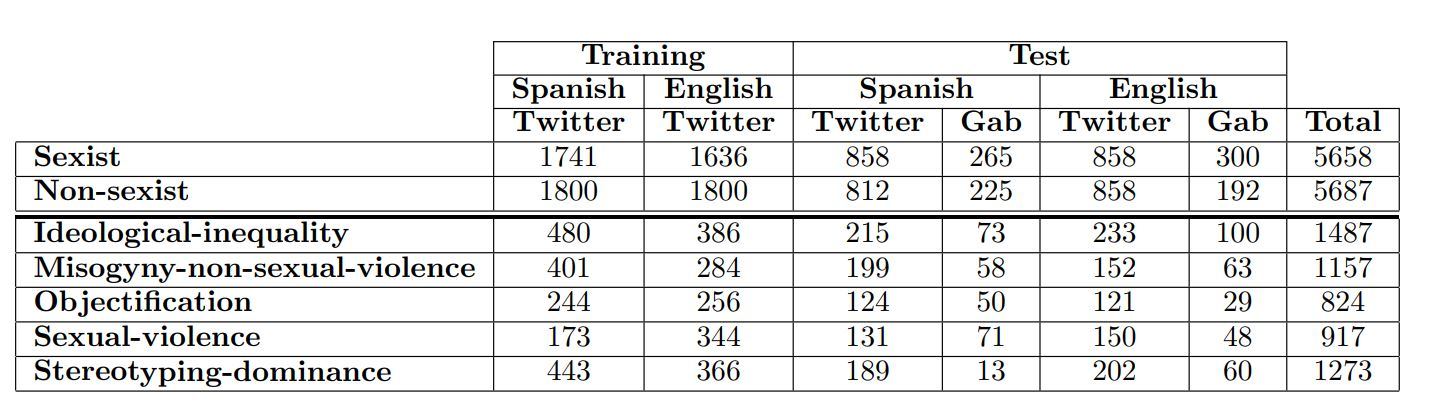
\includegraphics[width=16cm]{imagenes/Arte/dataset_exist2021.jpg}
    \caption{\centering Estadísticas del dataset de EXIST 2021)}
  \label{fig:dataset_exist2021}  
\end{figure}

Respecto a la primera tarea, se puede observar claramente que el dataset está balanceado en los dos idiomas, con 5.658 instancias sexistas y 5.687 instancias no sexistas. Por el otro lado, en la tarea 2, es posible observar algunas diferencias significativas en la distribución de algunas clases como se ejemplifica en la \autoref{fig:dataset_exist2021_task2} generada usando los datos anteriores:

\begin{figure}[H]
    \centering
    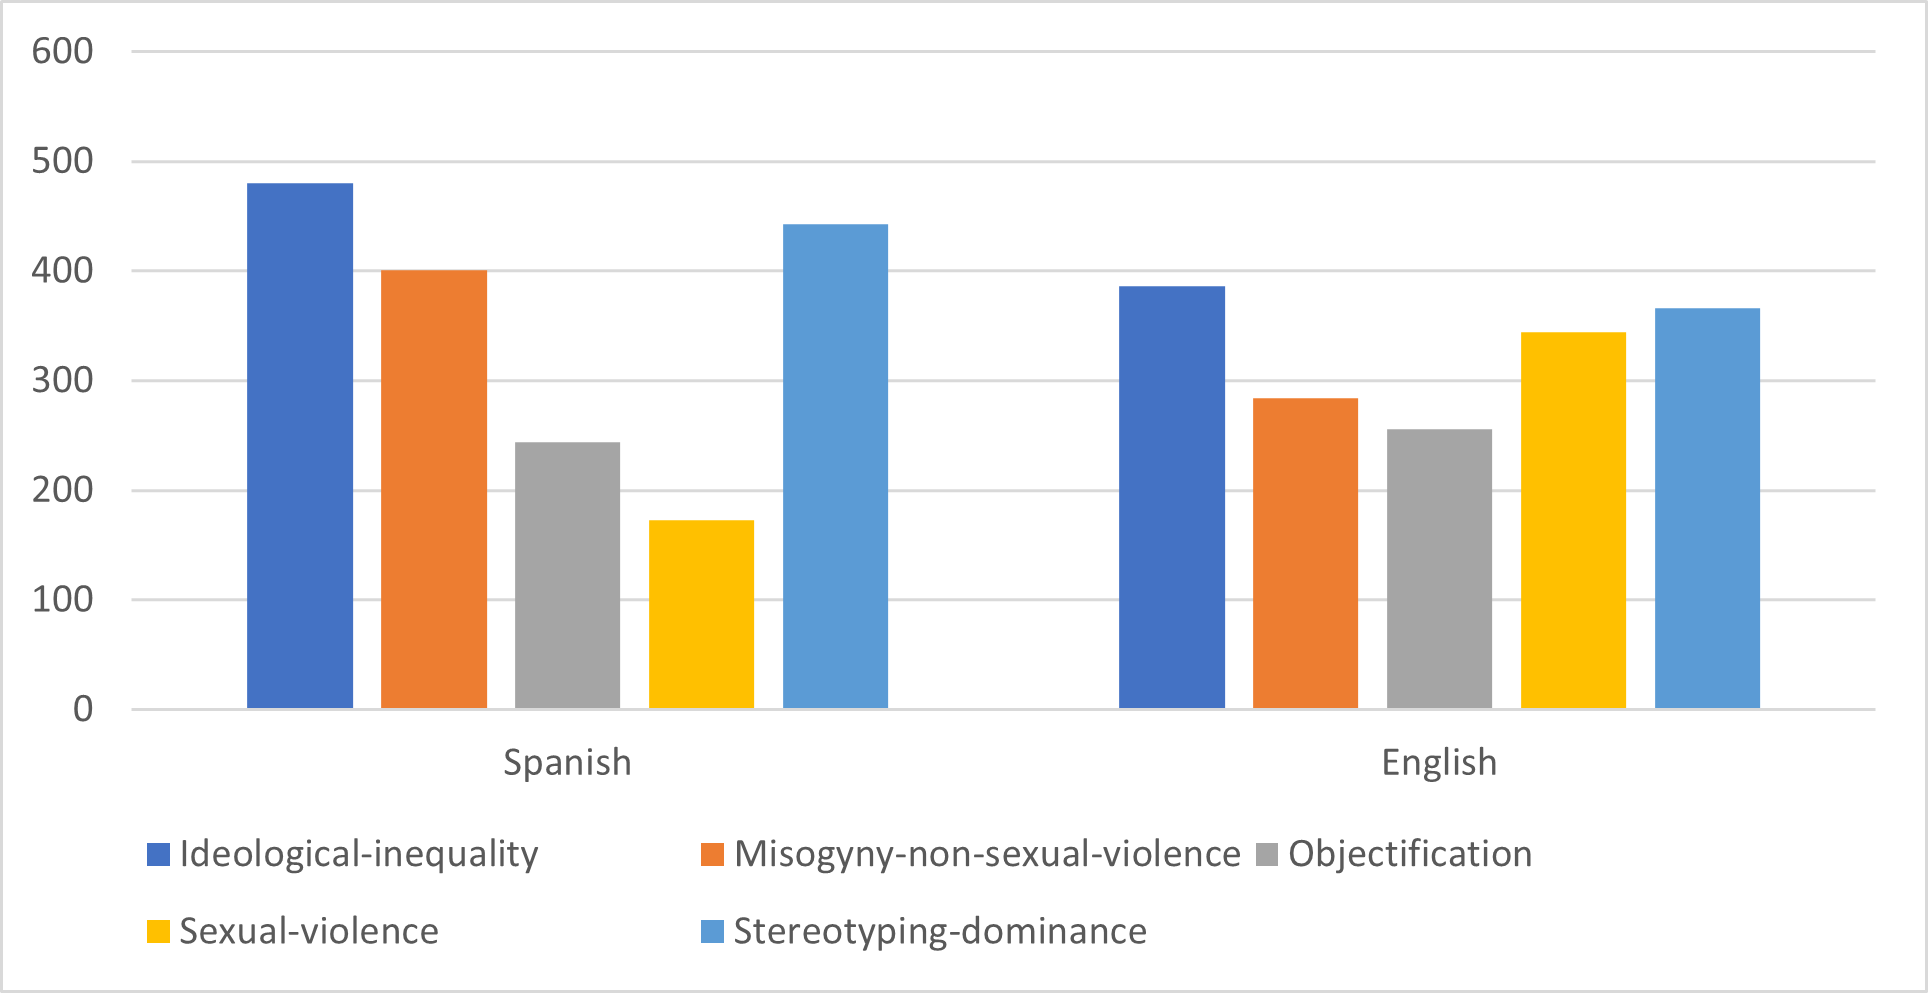
\includegraphics[width=16cm]{imagenes/Arte/task2_exist2021.png}
    \caption{\centering Distribución tarea 2 para EXIST 2021}
    \label{fig:dataset_exist2021_task2}  
\end{figure}

Se puede ver claramente que las diferentes clases están desbalanceadas entre sí. Por un lado, para los textos en español se observa que las clases mayoritarias son la clase de Ideología y desigualdad (480 instancias) y la clase estereotipos y dominancia (443 instancias) donde, por otro lado la clase minoritaria, Violencia-Sexual, posee 173 instancias.

De cara a los tweets en inglés, las instancias bajan para las clases mayoritarias y se equilibran algo más con las demás clases. En este caso la clase mayoritaria, siendo de nuevo Ideología y desigualdad, está compuesta de 386 instancias, lo que respecto de la instancia minoritaria, Objetificación , no supone una diferencia tan alta como para los tweets en español con 256 instancias.

Por otro lado, de cara a la competición en sí, se inscribieron un total de 76 equipos de 11 países diferentes tanto de Europa, Asia y América Del Norte. Sin embargo, solo presentaron modelos 31 equipos para la primera tarea y 27 para la segunda. La mayoría de los participantes se basaron en el uso de Transformers para las dos tareas. Un total de 14 equipos usaron BERT \cite{devlin2018bert} o mBERT (su versión multilingüe) \cite{pires2019multilingual}, 10 usaron una versión española llamada BETO \cite{de2021applying}, 5 RoBERTa \cite{liu2019roberta} y por último 4 equipos usaron una versión multilingüe de RoBERTa llamada XLM-RoBERTa \cite{lample2019cross}.

Además de transformadores algunos equipos usaron Support Vector Machines (SVM) \cite{rameshbhai2019opinion}, Random Forest (RF) \cite{antony2020dynamic}, Long Short Term Memory networks (LSTM) \cite{mostafa2022bidirectional}, Logistic Regresion(LR) \cite{vimal2020application} y con la librería FastText \cite{bhattacharjee2018fasttext}. Sin embargo, como se verá más adelante los modelos basados en Transformers resultaron ser en ambas tareas significativamente mejores.

De cara a los resultados para las diferentes tareas, hay que tener en cuenta que se evalúan desde varias perspectivas teniendo en cuenta el carácter multilingüe de la competición. Por un lado, se ofrecen los resultados para las pruebas realizadas sobre todos los datos (pruebas multilingües), y por otro lado se ofrecen por separado los resultados exclusivamente para los textos en español e inglés como si fueran dos tareas adicionales. Realmente el resultado que importa es el obtenido en la evaluación multilingüe pero los otros dos resultados son interesantes para observar por separado cómo funcionan los modelos planteados específicamente para cada idioma.

Cabe destacar que debido al desbalanceo de datos observado para la tarea 2, la métrica seleccionada para determinar el ganador fue el F1 en lugar del accuracy que fue seleccionado para determinar el ganador en la tarea 1, la cual recordando no se encontraba desbalanceada.

En general para la competición el equipo ganador para ambas tareas fue el equipo AI-UPV\_1. Este equipo utilizó el modelo BERT para los tweets en inglés y BETO para los tweets en español, así como mBERT como modelo multilingüe. Además, también utilizaron modelos de traducción automática para producir nuevos textos sintéticos tanto para inglés como español.

En la primera tarea, el equipo AI-UPV\_1 obtuvo un accuracy de 0.7668 y 0.7944 para inglés y español respectivamente. Así como un accuracy de 0.7804 para el test multilingüe compuesto de tanto los textos en español como en inglés.

Si bien quedó primero, para los resultados en inglés, quedó en tercer lugar por debajo de los equipos SINAI\_TL\_3 y multiaztertest\_1, que obtuvieron 0.7772 y 0.7717 para la tarea 1 en inglés. 

Es interesante mencionar que el equipo SINAI\_TL\_3 usó para la tarea en español BETO, mientras que para clasificar los textos en inglés usaron un modelo basado en la detección de polaridad \cite{sharma2014polarity} (análisis de sentimiento) creado con el dataset InterTASS \cite{martinez2018overview} obteniendo unos resultados de accuracy de 0.7772 y 0.7907 para las tareas de inglés y español respectivamente así como una accuracy global para la tarea 1 de 0.78 quedando en segundo lugar, justo por detrás de AI-UPV\_1.

Para la segunda tarea, el equipo AI-UPV\_1 obtuvo la primera posición para español (F1 de 0.6073), y terceros para inglés (F1 de 0.5507). Obteniendo la primera posición general para la tarea (multilingüe) con un F1 de 0.5787. 

Es interesante mencionar que el equipo que quedó primero en la subtarea en inglés, cuya única referencia accesible es su nombre LHZ\_1, usó un modelo mejorado de BERT y RoBERTa conocido como DeBERTa \cite{he2020deberta}, obteniendo unos resultados de F1 de 0.5604 y 0.5805 para las tareas en inglés y español respectivamente, obteniendo el segundo puesto en la clasificación general con un F1 de 0.5706.

En conclusión, para la competición EXIST 2021 el mejor resultado fue el ofrecido por el equipo AI-PV\_1 para ambas tareas, de 0.7804 de accuracy para la primera y 0.5787 de F1 para la segunda. Estos resultados se obtuvieron usando un sistema basado en varios modelos transformadores basados en BERT diferenciando entre los modelos usados para los textos en inglés y español consiguiendo así maximizar los resultados obtenidos al usar modelos más especializados en cada idioma.

%%%%%%%%%%%%%%%%%%%%%%%%%%%%%%%%%%%%%%%%%%%%%%%%%%%%%
%segunda parte: Exist 2022
%%%%%%%%%%%%%%%%%%%%%%%%%%%%%%%%%%%%%%%%%%%%%%%%%%%%%

Para la segunda entrega de la competición EXIST en 2022 las tareas se mantuvieron iguales, siendo detección del sexismo y clasificación del mismo dentro de las categorías ya mencionadas. De nuevo toda la información de la competición, así como resultados se obtienen directamente del paper relacionado con la misma \cite{rodriguez2022overview}.

Por otro lado, el dataset para esta competición, compuesto de un total de 12.390 instancias, si habría recibido algunos cambios respecto del de 2021. Si bien el dataset se obtenía mayoritariamente del usado para el año anterior, en esta edición se añadió también a la fase del training textos recogidos de la red social GAB \cite{zhou2019elites}, a diferencia de como se hizo en la anterior entrega donde solo se usaban esos textos en la fase de test.

El objetivo de esta modificación era comprobar si afectaría a los resultados de los modelos incluir contenido de una red social sin ningún tipo de control del contenido que se sube a ella durante la fase de entrenamiento.

A continuación se muestra la tabla de distribución de los datos obtenida del paper ya mencionado:

\begin{figure}[H]
    \centering
    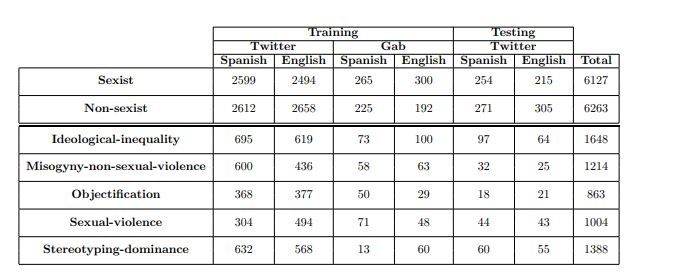
\includegraphics[width=16cm]{imagenes/Arte/dataset_exist2022.jpg}
    \caption{\centering Distribución del dataset para EXIST 2022}
\end{figure}

Si bien para el anterior año se han mostrado también el desbalanceo para la tarea 2, como se puede observar en la tabla ese desbalanceo sigue presente ya que la cantidad de entradas nuevas añadidas al dataset no tenían como objetivo arreglar ese problema y no presentan una proporción lo suficientemente grande del mismo. Es por esto por lo que no se incluye la gráfica al considerarse redundante. 

Al mantener el mismo desbalanceo que la entrega anterior, de cara a las métricas elegidas para determinar los ganadores no hubo cambios y se volvieron a usar accuracy para la tarea 1 y F1 para la tarea 2.

Una característica muy a tener en cuenta es que para esta entrega el set de test fue creado y evaluado por 6 expertos, 3 mujeres y 3 hombres para eliminar cualquier posible sesgo de género, por lo que se considera que la calidad de la anotación es significativamente mejor que la del año anterior.

De nuevo para este año el ganador para las dos tareas es el mismo, en este caso el ganador fue avacaondata\_1. Este equipo presentó para su mejor modelo una idea similar al ganador del año pasado con una unión de modelos, en este caso los modelos eran: BERTweet-large \cite{nguyen-etal-2020-bertweet}, RoBERTa y DeBERTa para los textos en inglés y BETO, BERTIN \cite{de2022bertin}, MarIA-base \cite{gutierrez2021spanish} y ROBERTuito para los textos en español. 

Con esta combinación de modelos obtuvo un accuracy de 0.7996 en la primera tarea bilingüe situándose en una mejora del estado del arte respecto del año pasado de un 0.0192 (2,4\% más). Por otro lado, a diferencia del año anterior este año los resultados en inglés fueron muy superiores con un 0.8422 de accuracy, un 0.065 más que el año anterior (8,36\% más) y para español algo peores que el año pasado con un 0.7801 de accuracy, lo cual lo sitúa 0.0143 por debajo (1,8\% menos). 

Concretamente para la tarea 1, de cara a los textos en español, quedó en 6 puesto obteniendo el ganador de esta subtarea un 0.7801 en accuracy usando una combinación de 10 modelos generados con RoBERTuito y otros 10 modelos generados con BERT usando una semilla diferente en cada entrenamiento de cada uno de los 20 modelos generados.

Es interesante destacar como la tarea en inglés ha mejorado tanto y por el contrario la tarea en español ha incluso empeorado respecto del estado del arte de un año a otro.

Para la segunda tarea, de nuevo ganador, con un 0.5106 de F1 score en los resultados generales lo cual supone una bajada en el estado del arte de 0.0681 (11,7\% menos) aún con una mejora ligera en la precisión del modelo.

Por otro lado, en los resultados específicos obtuvo un F1 de 0.5337 y 0.4867 para inglés y español respectivamente, siendo superado únicamente en los resultados en español por el equipo ELiRF-VRAIN\_3 el cual obtuvo un F1 de 0.4867 usando un de nuevo un sistema de modelos combinado de XLM-RoBERTa, RoBERTa y 3 modelos BERT para los textos en español y XLM-RoBERTa, RoBERTa, BERT, hateBERT \cite{ caselli2020hatebert} y ALBERT \cite{ lan2019albert} para los textos en inglés. 

Es decir, para esta segunda entrega de la competición de EXIST, el ganador y en general los primeros equipos, volvieron a usar un sistema compuesto por varios modelos de Transformer especializados en cada idioma siguiendo la tendencia del año pasado.

En cuanto a los resultados, se han observado mejoras algo bajas para la tarea 1 obteniendo por parte del ganador un accuracy de 0.7996 y peores para la tarea 2, obteniendo por parte del ganador un F1 de 0.5106. Sin embargo, de cara a la tarea 1 la detección de sexismo en inglés ha mejorado significativamente obteniendo un accuracy de 0.8422.

Se plantea una hipótesis acerca de los resultados obtenidos: En primer lugar, la mejora de un año para otro tampoco se puede esperar que sea excesiva y por otro este año, el set de test, solo el set de test que no entrenamiento, ha recibido un análisis mucho más profundo y exhaustivo por parte de 6 expertos. Estas dos razones pueden perfectamente ser la causa de los resultados tan variantes en las diferentes tareas e idiomas de cada una.

En general el estado del arte desde la perspectiva de la detección de sexismo en las redes sociales apunta a que los modelos Transformers pueden obtener resultados muy interesantes, al menos claramente mejores que sus contrapartes ya mencionadas, pero que hay espacio de mejora tanto en los propios modelos como en los datos que se usan para la tarea de entrenamiento. 

Como conclusión se ha observado una clara tendencia por parte de los mejores modelos a usar conocimiento de varios modelos a la vez y no depender exclusivamente de un modelo. Esta es una perspectiva interesante que plantear para futuros trabajos.